
%(BEGIN_QUESTION)
% Copyright 2007, Tony R. Kuphaldt, released under the Creative Commons Attribution License (v 1.0)
% This means you may do almost anything with this work of mine, so long as you give me proper credit

Shown here is the schematic diagram of a full ``PID'' analog pneumatic controller.  Although it lacks the features of output and setpoint tracking, it does possess all three control terms: Proportional, Integral, and Derivative.

$$\includegraphics[width=15.5cm]{i01636x01.eps}$$

Based on your analysis of this mechanism, answer the following questions:

\begin{itemize}
\item{} Is this controller reverse or direct acting?
\item{} Which valve adjusts the integral constant ($\tau_i$)?
\item{} Which valve adjusts the derivative constant ($\tau_d$)?
\item{} What will a change in the capacity tank's volume affect?
\item{} Will adjustment of the proportional constant affect either the integral or derivative responses?
\item{} What would happen if valve $V_2$ were fully shut?
\end{itemize} 

\vskip 20pt \vbox{\hrule \hbox{\strut \vrule{} {\bf Suggestions for Socratic discussion} \vrule} \hrule}

\begin{itemize}
\item{} A powerful problem-solving technique is performing a {\it thought experiment} where you mentally simulate the response of a system to some imagined set of conditions.  Describe a useful ``thought experiment'' for this system, and how the results of that thought experiment are helpful to answering these questions.
\end{itemize}

\underbar{file i01636}
%(END_QUESTION)





%(BEGIN_ANSWER)

{\bf Partial answer:}

\begin{itemize}
\item{}Which valve adjusts the derivative constant ($\tau_d$)?  {\bf V$_{2}$}
\item{}Will adjustment of the proportional constant affect either the integral or derivative responses?  {\bf Yes!}
\end{itemize} 

%(END_ANSWER)





%(BEGIN_NOTES)

{\it Is this controller reverse or direct acting?}

This controller is reverse-acting, because increases in PV result in decreases in Output.  An increase in the process variable signal will tend to rotate the lever clockwise about the fulcrum, thus increasing the flapper/nozzle gap and decreasing the output signal.
 
\vskip 10pt

{\it Which valve adjusts the integral constant ($\tau_i$)?}

Valve V$_{1}$, restricting the flow of air into and out of the upper bellows (opposite the feedback bellows).  Remember that the feedback bellows (labeled "P" for "proportioning" in Foxboro brand pneumatic controllers) will {\it always} act to increase the flapper/nozzle gap on an increase in output pressure, so that feedback will maintain flapper/nozzle gap relatively constant.  The bellows causing integral action (labeled "R" for "reset" in Foxboro brand pneumatic controllers) must always be {\it opposed} to the feedback bellows.  Thus, in this controller the lower bellows is the feedback bellows and the upper bellows is the integral or "reset" bellows.
 
\vskip 10pt

{\it Which valve adjusts the derivative constant ($\tau_d$)?}

Valve V$_{2}$, restricting the flow of air into and out of the lower bellows.  Following from the previous discussion of bellows identity, the lower bellows acts as both feedback ("proportioning") and derivative (rate) when there is a restriction between it and the source of output pressure.
 
\vskip 10pt

{\it What will a change in the capacity tank's volume affect?}

Changes in tank capacity will affect the $\Delta$volume/pressure relationship for the lower bellows.  This will impact the amount of {\it time} it takes for pressure to change in that bellows as a function of a given quantity of air moving into or out of the bellows.  Since the lower bellows performs the proportional and derivative responses, and because we know proportional action is time-independent, the volume must affect {\it derivative} (rate) response.
 
\vskip 10pt

{\it Will adjustment of the proportional constant affect either the integral or derivative responses?}

Yes, because changing the fulcrum position (the only proportional adjustment in this controller mechanism) will alter the mechanical advantage of the lever system, and this alters the input/output relationship between {\it all} bellows' forces.  Thus, changing this controller's proportional band results in both integral and derivative responses becoming more or less aggressive by the same factor.

\vskip 10pt

{\it What would happen if valve $V_2$ were fully shut?}

The gain of the controller would become infinite, because with the output bellows blocked off it could not balance any error from the PV/SP bellows.  The slightest change in PV and/or SP would cause the output to completely saturate.

 
\vskip 20pt \vbox{\hrule \hbox{\strut \vrule{} {\bf Virtual Troubleshooting} \vrule} \hrule}

This question is a good candidate for a ``Virtual Troubleshooting'' exercise.  Presenting the diagram to students, you first imagine in your own mind a particular fault in the system.  Then, you present one or more symptoms of that fault (something noticeable by an operator or other user of the system).  Students then propose various diagnostic tests to perform on this system to identify the nature and location of the fault, as though they were technicians trying to troubleshoot the problem.  Your job is to tell them what the result(s) would be for each of the proposed diagnostic tests, documenting those results where all the students can see.

During and after the exercise, it is good to ask students follow-up questions such as:

\begin{itemize}
\item{} What does the result of the last diagnostic test tell you about the fault?
\item{} Suppose the results of the last diagnostic test were different.  What then would that result tell you about the fault?
\item{} Is the last diagnostic test the best one we could do?
\item{} What would be the ideal order of tests, to diagnose the problem in as few steps as possible?
\end{itemize}


\vfil \eject

\noindent
{\bf Summary Quiz:}

Determine the effect of valve $V_1$ becoming completely plugged with debris:

$$\includegraphics[width=15.5cm]{i01636x02.eps}$$

\begin{itemize}
\item{} The output signal will fall to zero PSI
\vskip 5pt 
\item{} Gain will become infinite (huge)
\vskip 5pt 
\item{} The control action will switch from reverse to direct
\vskip 5pt 
\item{} Derivative action will become zero minutes
\vskip 5pt 
\item{} The capacity tank will burst from excess pressure
\vskip 5pt 
\item{} Integral action will become zero repeats per minute
\end{itemize}

%INDEX% Control, proportional + integral + derivative: pneumatic controller

%(END_NOTES)


